\documentclass[14pt, aspectratio=169]{beamer}
\usetheme{Copenhagen}
\usecolortheme{beaver}

\setbeamertemplate{navigation symbols}{}

\title{2D Rogue-Like}
\author{Team Cherry}
\date{2022/11/03}

\begin{document}
	\maketitle
	\begin{frame}{Csapattagok}
		\begin{itemize}
			\item Orosz Péter
			\item Dobai Attila
			\item Drahos Alinka
			\item Tőzsér Zétény
			\item Gáncsos Dániel
		\end{itemize}
	\end{frame}
	
	\begin{frame}{Áttekintés}
		\begin{block}{Legfontosabb funkciók}\end{block}
		\begin{block}{Használhatóság}\end{block}
		\begin{block}{Teljesítmény}\end{block}
		\begin{block}{Felhasznált kész komponenesek}\end{block}
	\end{frame}
		
	\begin{frame}{Legfontosabb funkciók}
		\only<1>
		{
			\begin{figure}
    			\centering
    			\textbf{Játékos - Boltos Interakcó}\par\medskip
    			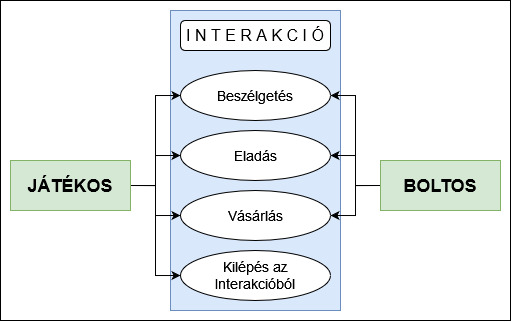
\includegraphics[height = 0.6\textheight]{jatekos-boltos.jpg}
			\end{figure}
		}
		\only<2>
		{
			\begin{figure}
    			\centering
    			\textbf{Játékos - Ellenfél Interakcó}\par\medskip
    			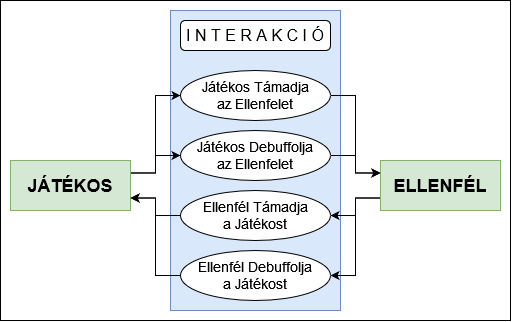
\includegraphics[height = 0.6\textheight]{jatekos-ellenfel.jpg}
			\end{figure}
		}
		\only<3>
		{
			\begin{figure}
    			\centering
    			\textbf{Játékos - Tárhely Interakcó}\par\medskip
    			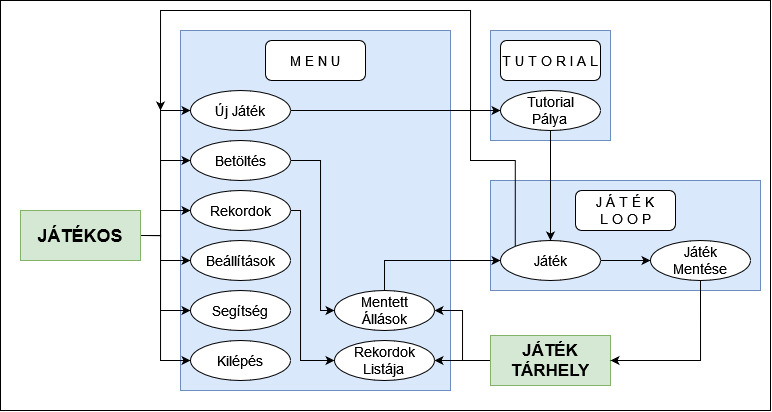
\includegraphics[height = 0.6\textheight]{jatekos-tarhely.jpg}
			\end{figure}
		}
	\end{frame}
	
	\begin{frame}{Használhatóság}
		\begin{itemize}
			\item Több választható nehézségi fokozat
			\item Tutorial pálya a játék alapvető funkcióinak a megismerésére
			\item Színvakok számára külön opció hogy hozzáférhetőbb legyen egy nagyobb közönségnek.
		\end{itemize}
	\end{frame}
	
	\begin{frame}{Teljesítmény}
		A játék tudatosan alacsony teljesítmény igénnyel készül hogy minnél nagyobb közönséget el tudjunk érni vele. A minimum rendeszerigény a kovetkező lesz:
		\begin{itemize}
			\item Intel Core i3-3225 
			\item 4GB memória
			\item GTX 650 GPU
			\item 2GB szabad tárhely
		\end{itemize}
	\end{frame}
	
	\begin{frame}{Felhasznált kész komponenesek}
		\begin{itemize}
			\item javax.swing.* - GUI, TileSet, Sprite -ra lesznek felhasználva.
			\item javax.sound.* - Minden hang és effekt -re ezt a könyvtárat fogjuk használni.
		\end{itemize}
	\end{frame}
\end{document}